\documentclass[11pt]{article}

\usepackage[a4paper,margin=1in]{geometry}
\usepackage[T1]{fontenc}
\usepackage{lmodern}
\usepackage{microtype}
\usepackage{amsmath,amssymb}
\usepackage{array}
\usepackage{booktabs}
\usepackage{longtable}
\usepackage{tabularx}
\usepackage{xcolor}
\usepackage{hyperref}
\usepackage{enumitem}
\usepackage{tikz}
\usetikzlibrary{arrows.meta,positioning,shapes.geometric,fit,backgrounds,calc}

\hypersetup{
  colorlinks=true,
  linkcolor=blue!55!black,
  citecolor=blue!55!black,
  urlcolor=blue!55!black
}

\definecolor{ppBlue}{RGB}{33,79,140}
\definecolor{ppGreen}{RGB}{30,120,90}
\definecolor{ppGold}{RGB}{172,122,35}
\definecolor{ppRed}{RGB}{178,72,72}
\definecolor{ppGray}{RGB}{246,248,250}
\definecolor{ppLine}{RGB}{88,98,112}

\newcommand{\code}[1]{\texttt{#1}}
\newcommand{\sui}{\textsc{Sui}}
\newcommand{\walrus}{\textsc{Walrus}}
\newcommand{\pprf}{\code{PPRF}}

\title{\textbf{PaperProof Whitepaper}\\
\large A Protocol for Durable Digital Artifacts on Sui and Walrus}
\author{PaperProof Labs\\\href{mailto:paperproof.labs@gmail.com}{paperproof.labs@gmail.com}}
\date{Draft v0.1 \\ May 2026}

\begin{document}
\maketitle

\section*{Copyright and Use Notice}

Copyright \copyright{} 2026 PaperProof Labs. All rights reserved.

This whitepaper is published for review, discussion, education, ecosystem
coordination, and integration with the official PaperProof Protocol deployments.
Readers may download, print, cite, and quote limited portions of this document
for those purposes. This document does not grant rights to use the PaperProof
name, PaperProof Labs name, logos, trademarks, official deployment identity, or
official manifests in a confusing or misleading manner. It does not relicense
the PaperProof smart contracts, SDKs, website, marks, or other project
materials, which remain governed by their own license notices.

This whitepaper is not an investment prospectus, financial promotion, promise of
returns, legal opinion, or guarantee of protocol adoption. It describes a
protocol direction, current implementation posture, and intended ecosystem path.
Future governance, fees, incentives, and roadmap items are directional and may
change through development, security review, community feedback, and applicable
governance processes.

\begin{abstract}
Important digital works increasingly move across unstable boundaries: storage
links, social posts, repositories, preprint pages, datasets, software releases,
chat archives, and application databases. These surfaces are useful, but none of
them alone gives the work itself a neutral, durable, verifiable, and composable
protocol identity.

PaperProof is a Sui-native protocol for durable digital artifacts backed by
Walrus content storage \cite{sui_platform,walrus_storage}. It treats a work not as a single uploaded file, but as an
artifact series: a continuing object with typed versions, content commitments,
official comments, likes, governance-aware parameters, canonical events, and
developer-facing SDKs. The goal is not to replace academic archives, software
platforms, storage networks, social media, or community forums. The goal is to
give important digital works a protocol layer beneath and beside those systems.

This whitepaper explains the vision, user value, ecosystem role, developer
surface, governance direction, PPRF relevance, sustainability principles,
roadmap, and risks of PaperProof. Detailed object structures, error codes, and
event fields belong in the yellow paper; formal system analysis belongs in the
academic paper. This document is the ecological argument: why PaperProof should
exist, who can build on it, and how it can grow without pretending to solve every
social, financial, or editorial problem at launch.
\end{abstract}

\tableofcontents
\newpage

\section{Executive Summary}

PaperProof is a protocol for durable, verifiable, and community-readable digital
artifacts. A PaperProof artifact may be a preprint, blog post, technical report,
dataset, software release, or generic file. The artifact's large content lives
on \walrus{}, while its protocol identity and lifecycle live on \sui{}.

The central idea is simple: important works deserve more than a file link and an
application page. They should have an identity that can survive frontend changes,
repository migrations, social-feed decay, organizational changes, and market
cycles. That identity should support versions, content verification, official
interaction objects, events for indexers, and enough structure for applications
and agents to interpret the work safely.

PaperProof begins with a practical implementation rather than only a thesis. It
has mainnet contracts, a deployment manifest, an official static application,
TypeScript, Python, and Rust SDKs, Walrus content helpers, governance flows,
query and watch surfaces, and documentation. These pieces form a small but real
protocol seed.

\subsection{The Short Version}

\begin{itemize}[leftmargin=*]
  \item PaperProof gives digital artifacts durable protocol identities.
  \item Sui stores compact authoritative state; Walrus stores large content.
  \item Artifact series support typed versions instead of one-off uploads.
  \item Official comments and likes are bound to artifact objects.
  \item PPRF is used for governance and protocol participation signals.
  \item SDKs make PaperProof usable from frontend apps, scripts, notebooks, and indexers.
  \item PaperProof is open to third-party apps; the official website is only one entrance.
  \item Governance, fees, incentives, and community operations are intended to grow gradually.
\end{itemize}

\section{The Problem: Digital Works Without Protocol Identity}

Digital works are everywhere, but their identities are fragmented. A paper may
be on a preprint server. A dataset may be in one storage system. A software
release may be on a repository host. A protocol article may be in a blog. A
discussion may happen on social media. Years later, the links, accounts,
websites, and application databases around the work may have changed.

This creates a gap between the content and its public life. A file hash can
identify bytes, but it does not describe the artifact's type, owner, version
lineage, official comments, likes, governance history, or canonical event stream.
A web page can provide context, but it usually belongs to one application
operator. A repository release can be useful, but it is not a neutral protocol
identity. A social post can create attention, but it is not durable
infrastructure.

PaperProof addresses this missing layer. It asks: what if a digital work could
have a durable identity independent of one frontend, while still remaining easy
to use from ordinary applications?

\subsection{Why This Matters}

Durable artifact identity matters because modern knowledge is not static. A
preprint may gain new versions. A dataset may be reused by another project. A
software release may need verifiable package references. A technical report may
become governance evidence. A blog post may become part of a community's memory.
A forum thread may host long-term discussion around a protocol artifact.

Without protocol identity, every application rebuilds its own partial truth. One
system knows where the file is. Another knows the comments. Another knows the
versions. Another knows the author. Another knows the community reaction. The
artifact itself remains scattered.

\section{The PaperProof Vision}

PaperProof's vision is to become a durable artifact identity layer for Sui and
Walrus. It should be small enough to survive, structured enough to integrate,
and open enough for communities to build multiple applications on top of it.

The first official application is not meant to be the only PaperProof
application. It is a reference interface: Explore, Publish, Governance, My Space,
Docs, Blog, Forum, and PaperProof Copilot. Other people should be able to build
their own portals, dashboards, indexers, notebooks, mobile apps, institutional
archives, community forums, and agentic workflows using the same protocol facts.

\begin{figure}[h]
\centering
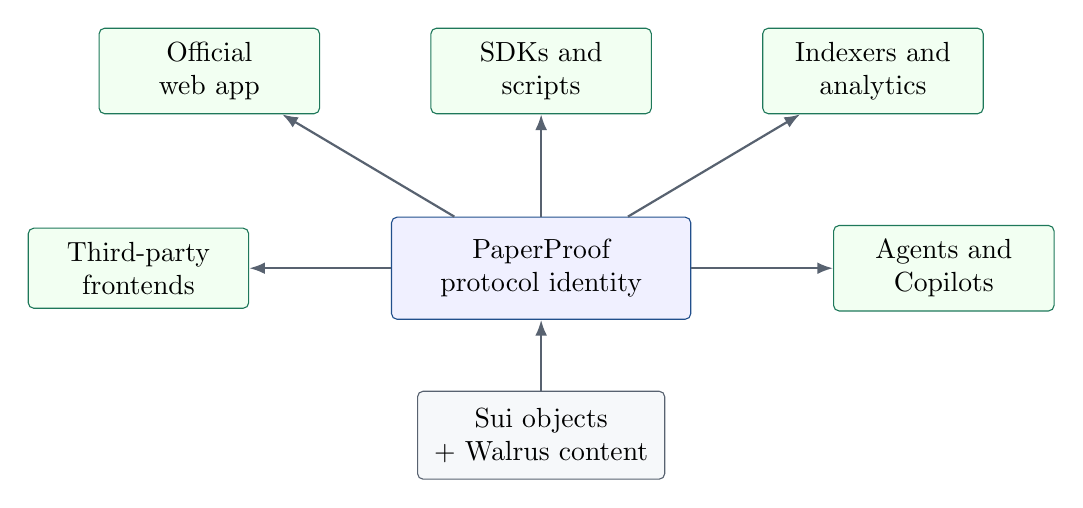
\begin{tikzpicture}[
  node distance=9mm,
  box/.style={draw=ppLine, rounded corners=2pt, fill=ppGray, align=center, inner sep=6pt, minimum width=31mm},
  core/.style={draw=ppBlue, rounded corners=2pt, fill=blue!6, align=center, inner sep=8pt, minimum width=38mm},
  app/.style={draw=ppGreen, rounded corners=2pt, fill=green!5, align=center, inner sep=5pt, minimum width=28mm},
  arr/.style={-{Latex[length=2mm]}, thick, draw=ppLine}
]
\node[core] (protocol) {PaperProof\\protocol identity};
\node[box, below=of protocol] (suiwalrus) {Sui objects\\+ Walrus content};
\node[app, above left=13mm and 9mm of protocol] (official) {Official\\web app};
\node[app, above=13mm of protocol] (sdk) {SDKs and\\scripts};
\node[app, above right=13mm and 9mm of protocol] (indexer) {Indexers and\\analytics};
\node[app, right=18mm of protocol] (agents) {Agents and\\Copilots};
\node[app, left=18mm of protocol] (third) {Third-party\\frontends};
\draw[arr] (suiwalrus) -- (protocol);
\draw[arr] (protocol) -- (official);
\draw[arr] (protocol) -- (sdk);
\draw[arr] (protocol) -- (indexer);
\draw[arr] (protocol) -- (agents);
\draw[arr] (protocol) -- (third);
\end{tikzpicture}
\caption{PaperProof is intended as a protocol layer, not a single website.}
\label{fig:vision}
\end{figure}

\subsection{What PaperProof Should Become}

PaperProof should become:

\begin{itemize}[leftmargin=*]
  \item a durable coordinate system for digital artifacts;
  \item a publishing and versioning layer for works that need public commitments;
  \item a content gateway that makes Walrus easier to use in artifact workflows;
  \item an event surface for indexers, analytics, and community applications;
  \item a developer platform with SDKs in multiple languages;
  \item a governance-aware substrate for protocol evolution;
  \item a foundation for agent-readable artifact workflows.
\end{itemize}

\subsection{What PaperProof Should Not Become}

PaperProof should not pretend to be everything. It should not become a monolithic
social network, a full academic review authority, a universal storage network, a
centralized repository host, a legal compliance oracle, or a guaranteed reward
machine. Its core job is to record durable facts around artifacts. Communities,
applications, reviewers, developers, and markets can interpret those facts.

\section{What Is a PaperProof Artifact?}

A PaperProof artifact is a continuing protocol object, not merely a file. It has
a series identity, one artifact type, a human-readable artifact code, an owner,
one or more typed versions, content commitments, Walrus references, official
comments, official likes, status fields, timestamps, and events.

\subsection{Artifact Series}

The series is the continuing identity. A software project may have many releases.
A preprint may have revised versions. A dataset may be corrected. A technical
report may become more complete. A blog post may receive a canonical update. A
generic file may be replaced by a clearer version. PaperProof models these as
versions under one series rather than unrelated uploads.

\subsection{Typed Versions}

The six initial artifact types are:

\begin{table}[h]
\centering
\caption{Initial PaperProof artifact types.}
\begin{tabularx}{\textwidth}{p{0.25\textwidth}X}
\toprule
\textbf{Type} & \textbf{Typical use} \\
\midrule
\code{preprint} & Manuscripts, research drafts, academic-style papers. \\
\code{blog\_post} & Protocol announcements, community posts, essays, official updates. \\
\code{technical\_report} & Design notes, audits, specifications, engineering reports. \\
\code{dataset} & Data archives, schemas, reproducibility packages, research data. \\
\code{software\_release} & Source archives, package hashes, changelogs, release records. \\
\code{generic\_file} & Miscellaneous files that do not yet need a specialized type. \\
\bottomrule
\end{tabularx}
\end{table}

These types are intentionally limited. Type scarcity helps SDKs, indexers,
frontends, and governance understand what a record means. User-facing labels,
communities, tags, and themes can be flexible at the application layer, but
protocol-recognized types should remain stable and governable.

\section{Why Sui and Walrus}

PaperProof depends on two complementary foundations.

\sui{} provides object-centric protocol state. PaperProof objects map naturally
to Sui's model: artifact series, type registries, typed version records,
comments trees, likes books, governance vaults, fee managers, proposals, and
votes. This object model helps the protocol represent relationships explicitly
instead of hiding them inside one application database \cite{sui_platform,sui_move}.

\walrus{} provides storage for large content. PDFs, datasets, source archives,
images, long comments, and static sites should not be stored as large on-chain
objects. Walrus lets PaperProof keep content available while Sui records compact
commitments, references, and state transitions \cite{walrus_storage}.

Together, Sui and Walrus make PaperProof possible as a living artifact protocol:
transactions can represent meaningful artifact actions, while large content
remains in a storage layer designed for that role.

\section{Protocol Layers}

PaperProof can be understood as five layers:

\begin{enumerate}[leftmargin=*]
  \item Content layer: Walrus blobs and static sites.
  \item Protocol state layer: Sui objects and Move contracts.
  \item Event layer: canonical events for applications and indexers.
  \item Developer layer: SDKs, examples, query providers, watch APIs, and CLIs.
  \item Application layer: official app, third-party sites, forums, dashboards, agents, and data tools.
\end{enumerate}

This layering is important. The protocol does not need every future product
feature in the Move contracts. It needs stable facts. Applications can build
different experiences around those facts.

\section{Official App and Open Entry Points}

The official PaperProof web application is a reference interface. It helps users
explore artifacts, publish new works, add versions, read details, comment, like,
vote, claim locked funds, view wallet state, browse docs, read official posts,
and participate in forums.

But the official app is not the protocol's only entrance. A university group
could build a research portal. A software community could build a release
dashboard. A data team could build an analytics indexer. A mobile developer
could build a lightweight artifact browser. An AI developer could build an agent
that summarizes artifact histories and governance proposals. A wallet could show
PaperProof-related objects and transactions natively.

\subsection{Official Does Not Mean Exclusive}

PaperProof Labs may operate official deployments, official manifests, official
docs, and an official website. That gives the ecosystem a trusted starting
point. It should not prevent truthful third-party integrations. Third-party
applications should be free to build on official PaperProof deployments as long
as they do not misrepresent themselves as official or confuse users about
authority.

\section{SDK and Developer Ecosystem}

PaperProof provides three SDK tracks with different personalities.

\begin{table}[h]
\centering
\caption{SDK roles.}
\begin{tabularx}{\textwidth}{p{0.18\textwidth}X}
\toprule
\textbf{SDK} & \textbf{Primary role} \\
\midrule
TypeScript & Frontend and Node.js integration, browser-wallet workflows, transaction builders, query providers, watch APIs, ContentService. \\
Python & Scripts, notebooks, batch queries, CSV/JSON exports, operational tooling, research analysis, simple automation. \\
Rust & High-performance indexers, checkpoint ingestion, persistent cursors, database sinks, backend services, enterprise-style data infrastructure. \\
\bottomrule
\end{tabularx}
\end{table}

This split is deliberate. A browser developer, a data analyst, and an indexer
operator do not need the same interface. The protocol should feel natural in
each environment.

\subsection{Developer Goals}

PaperProof SDKs should make common actions short and safe:

\begin{itemize}[leftmargin=*]
  \item load the active deployment manifest;
  \item query recent artifacts;
  \item read artifact details and versions;
  \item build transactions without executing them;
  \item execute with browser wallet or keypair;
  \item parse typed transaction results;
  \item handle provider failure honestly;
  \item query comments, likes, proposals, and voting records;
  \item publish, read, verify, extend, and transfer Walrus content through a simplified ContentService;
  \item watch canonical events without accepting look-alike package events.
\end{itemize}

\section{Indexers, Data Services, and Watchers}

Long-term protocols need data infrastructure. PaperProof events should be
available to frontends, explorers, dashboards, research tools, and community
applications. But events must be interpreted carefully. A raw event name is not
enough. Indexers must verify package IDs, registry IDs, root bindings, series
bindings, comments tree IDs, likes book IDs, and governance config bindings.

The Rust SDK is designed to make this path stronger. It can support
checkpoint-oriented ingestion, persistent cursors, idempotent event IDs,
SQLite/Postgres sinks, backfill, tail mode, metrics, and deployment drift
policies. This is the path from a working protocol to a dependable data
ecosystem.

\section{PaperProof Copilot and Agentic Interfaces}

PaperProof Copilot is a browser-side assistant pattern. It can read structured
page data, protocol prompts, and visible state to explain what users are seeing.
It can clarify artifact details, voting state, locked funds, publish forms,
comment behavior, and safety checks.

Copilot does not sign transactions. It does not hold private keys. It does not
replace the wallet. This separation is central to PaperProof's Agentic Web
position: AI can help users understand and prepare actions, but authorization
should remain with human-approved wallets and Sui object permissions.

PaperProof artifacts are suitable for agentic workflows because they are
structured. Agents can read types, versions, comments, proposals, and events
instead of scraping arbitrary pages. This opens the door to artifact summaries,
research assistants, governance explainers, indexer diagnostics, and content
maintenance agents.

\section{PPRF Utility and Governance Direction}

\pprf{} is the PaperProof governance and participation asset. It currently
supports governance voting and proof-of-holding participation signals such as
likes. It is not a guarantee of revenue, yield, adoption, or content quality.

\subsection{Governance Philosophy}

PaperProof should not pretend to be fully decentralized on day one. Early-stage
protocols need security response, deployment discipline, SDK updates, frontend
repair, manifest maintenance, and practical recovery paths. The right path is
progressive decentralization: begin with accountable early maintenance, then
move more parameters and authority into transparent governance as the protocol,
community, and tooling mature.

\subsection{Early Governance Scope}

Early governance should focus on limited, high-signal parameters:

\begin{itemize}[leftmargin=*]
  \item fee levels;
  \item artifact type enablement;
  \item governance configuration;
  \item action enablement;
  \item operator and authority transitions;
  \item direct authority reduction over time;
  \item future type activation.
\end{itemize}

This scope is intentionally conservative. Governance should first protect the
protocol from obvious parameter abuse and centralization risk. It should not
rush into complicated financial promises or vague reward mechanics.

\section{Fees, Sustainability, and Anti-Spam}

Fees in PaperProof are primarily resource and spam boundaries. They are not
designed as a maximized revenue extraction system. Publishing, adding versions,
and comments can carry fees configured through governance-aware mechanisms.
Fees may be low or even zero in some periods, but the protocol still needs
bounded metadata, object binding, status checks, and canonical filters.

Sustainability should develop gradually. In early phases, PaperProof Labs may
carry much of the maintenance burden. Over time, the ecosystem may need grants,
bounties, infrastructure funding, content-maintenance policies, and contributor
support. These mechanisms should be transparent, modest, and auditable before
they become ambitious.

\section{Incentives and Community Growth}

PaperProof should avoid promising simplistic ``publish-to-earn'' incentives.
Artifact quality, research value, social usefulness, and software reliability
cannot be produced by token rewards alone. Bad incentives can fill a protocol
with spam faster than good content.

Instead, early incentives should support useful ecosystem work:

\begin{itemize}[leftmargin=*]
  \item SDK examples and integrations;
  \item indexers and dashboards;
  \item documentation and translations;
  \item official and community blog posts;
  \item artifact curation and educational collections;
  \item frontend experiments;
  \item tools for Walrus content maintenance;
  \item agents that help users understand protocol state safely.
\end{itemize}

The community should grow around credible artifacts and useful tools, not only
around token speculation. PPRF governance can become meaningful only if there is
an ecosystem worth governing.

\section{Roadmap}

The roadmap is directional, not a promise of dates, returns, or specific token
incentives.

\subsection{Phase 0: Mainnet Protocol Seed}

The seed phase establishes the minimum durable protocol:

\begin{itemize}[leftmargin=*]
  \item mainnet contracts for publishing, comments, likes, governance, and fees;
  \item initial artifact types;
  \item official deployment manifest;
  \item TypeScript, Python, and Rust SDKs;
  \item official static web application;
  \item yellow paper, academic paper, slides, and developer documentation;
  \item opt-in mainnet integration scripts and examples.
\end{itemize}

\subsection{Phase 1: Usable Protocol Surface}

This phase focuses on making PaperProof pleasant and credible for early users:

\begin{itemize}[leftmargin=*]
  \item polish Explore, Publish, Governance, My Space, Docs, Blog, and Forum;
  \item strengthen PaperProof Copilot;
  \item improve Walrus upload/read/verify/extend/transfer flows;
  \item improve examples and tutorials;
  \item harden query providers and watch APIs;
  \item clarify user safety, wallet prompts, and error explanations.
\end{itemize}

\subsection{Phase 2: Developer and Data Ecosystem}

This phase expands beyond the official website:

\begin{itemize}[leftmargin=*]
  \item third-party frontends and research portals;
  \item high-performance indexers;
  \item analytics dashboards;
  \item notebook and CLI workflows;
  \item CSV/JSON export tools;
  \item event subscriptions and watcher services;
  \item grants or bounty experiments for useful ecosystem work.
\end{itemize}

\subsection{Phase 3: Governance Expansion}

Governance can grow as the protocol becomes more used:

\begin{itemize}[leftmargin=*]
  \item more parameter changes through PPRF proposals;
  \item clearer treasury or ecosystem-support policy if needed;
  \item transparent upgrade procedures;
  \item stronger role-transition processes;
  \item gradual reduction of direct authority;
  \item community-led proposals for new artifact types or application standards.
\end{itemize}

\subsection{Phase 4: Durable Knowledge Network}

The long-term ambition is a multi-entry artifact network:

\begin{itemize}[leftmargin=*]
  \item multiple frontends and community portals;
  \item multiple indexers and data services;
  \item academic, open-source, dataset, protocol-documentation, and community publishing use cases;
  \item agent-readable artifact histories;
  \item long-lived content and governance records on Sui and Walrus;
  \item PaperProof as a recognized digital artifact identity layer.
\end{itemize}

\section{Risk, Safety, and Non-Guarantees}

PaperProof makes artifact commitments more durable and verifiable. It does not
make every artifact true, original, legal, useful, safe, or valuable. A bad paper
can be published. A misleading dataset can be uploaded. A spam comment can be
posted. A token vote can be apathetic or concentrated. A frontend can still have
bugs. A storage lifecycle can still require maintenance.

\subsection{User and Developer Risks}

Users should understand wallet prompts before signing. Developers should apply
canonical event filters and drift checks. Indexers should distinguish failed
queries from empty state. Frontends should not report ``no comments'' or ``no
votes'' when provider reads failed. Agents should explain uncertainty rather
than inventing confidence.

\subsection{Governance Risks}

Governance can be captured, ignored, or misunderstood. Token voting is a
mechanism, not wisdom. PaperProof governance should remain transparent about
payloads, vote totals, locked funds, claim state, execution status, and authority
boundaries.

\subsection{Economic Non-Guarantees}

This whitepaper does not promise token price, returns, liquidity, listing,
revenue, grants, airdrops, user growth, or commercial success. Fees and
incentives are protocol tools, not guarantees.

\section{Conclusion}

PaperProof begins with a simple belief: important digital works deserve durable
protocol identities. Not every file needs this. Not every post should become
protocol state. But some artifacts matter enough that their identity, versions,
content commitments, interactions, governance records, and event history should
outlive a single application.

Sui and Walrus make this practical. Sui provides object-centric state and cheap
transactions. Walrus provides large content storage and static application
surfaces \cite{sui_platform,sui_move,walrus_storage}. PaperProof connects them into an artifact protocol with SDKs, indexers,
frontends, and agent-readable workflows.

The official PaperProof application is only the first doorway. The larger goal is
an ecosystem where researchers, developers, communities, data users, indexer
operators, and agent builders can all treat PaperProof artifacts as durable
public objects. If that ecosystem grows carefully, PaperProof can become a small
but resilient layer for digital knowledge on Sui and Walrus.

\begin{thebibliography}{10}

\bibitem{sui_platform}
Mysten Labs.
\newblock \emph{The Sui Smart Contracts Platform}.
\newblock 2022. \url{https://docs.sui.io/doc/sui.pdf}

\bibitem{sui_move}
Adam Welc and Sam Blackshear.
\newblock ``Sui Move: Modern Blockchain Programming with Objects.''
\newblock In \emph{Companion Proceedings of the 2023 ACM SIGPLAN International Conference on Systems, Programming, Languages, and Applications: Software for Humanity}, pages 53--55, 2023.
\newblock doi: 10.1145/3618305.3623605.

\bibitem{walrus_storage}
George Danezis, Giacomo Giuliari, Eleftherios Kokoris Kogias, Markus Legner, Jean-Pierre Smith, Alberto Sonnino, and Karl W{\"u}st.
\newblock ``Walrus: An Efficient Decentralized Storage Network.''
\newblock arXiv:2505.05370, 2025. \url{https://arxiv.org/abs/2505.05370}

\bibitem{ipfs}
Juan Benet.
\newblock ``IPFS - Content Addressed, Versioned, P2P File System.''
\newblock arXiv:1407.3561, 2014. \url{https://arxiv.org/abs/1407.3561}

\bibitem{filecoin}
Protocol Labs.
\newblock \emph{Filecoin: A Decentralized Storage Network}.
\newblock 2017. \url{https://filecoin.io/filecoin.pdf}

\bibitem{arweave}
Sam Williams, Viktor Diordiiev, Lev Berman, India Raybould, and Ivan Uemlianin.
\newblock \emph{Arweave: A Protocol for Economically Sustainable Information Permanence}.
\newblock 2023. \url{https://www.arweave.org/yellow-paper.pdf}

\bibitem{desci_values}
Lukas Weidener and Cord Spreckelsen.
\newblock ``Decentralized science (DeSci): definition, shared values, and guiding principles.''
\newblock \emph{Frontiers in Blockchain}, 7:1375763, 2024.
\newblock doi: 10.3389/fbloc.2024.1375763.

\bibitem{blockchain_open_science}
Krzysztof Janowicz, Blake Regalia, Pascal Hitzler, Gengchen Mai, Stephanie Delbecque, Maarten Fr{\"o}hlich, Patrick Martinent, and Trevor Lazarus.
\newblock ``On the prospects of blockchain and distributed ledger technologies for open science and academic publishing.''
\newblock \emph{Semantic Web}, 9(5):545--555, 2018.
\newblock doi: 10.3233/SW-180322.

\end{thebibliography}

\end{document}
